\documentclass[11pt]{article}

% The algorithm looks way better with the default wider layout (the default
% layout also leads to more pages)
%\usepackage{acl2016}
%\usepackage{times}
\usepackage{url}
\usepackage{latexsym}
\usepackage{amsmath,amssymb}
\usepackage{algorithm}
\usepackage{algpseudocode}
\usepackage{graphicx}
\usepackage{subfig}
\usepackage{natbib,textcomp}
%\aclfinalcopy

\title{Unsupervised Word Segmentation}
\author{Maarten de Jonge \and Pepijn Kokke \and Edwin Odijk}
\date{}

%NOTE: the report has a page requirement of 7-8 pages. It sounds more like a guideline though, because the TAs seem like decent people.
%literal copypasta from the ULL page: "The report for the first assignment on Bayesian methods should be short (7-8 pages)."

\begin{document}

\maketitle

\begin{abstract}
%Probably best to save this for last.
% - why would we do word segmenation
% - where did we get it from (Goldman)
% - what do we do (model based on MBDP-1, unigram, gibbs sampling
% - how did we implement it (any noteworthy things about it)
% - experiments
% - results
% - conclusion
\end{abstract}

\section{Introduction}
%Intro looks done-ish? There's still a couple of refs in here that I didn't bother fixing right away. It's (REF.GOLDMAN) right now.
%If we want to pad here, we can just repeat some of the stuff from the Method section
As we grow up, we quickly pick up the language spoken in our direct environment. Not only as infants, but also in our later lives can we learn different languages. Doing so is not trivial, however, and one of the problems we have to overcome is that of discerning the individual words from a spoken sentence. We may be able to do so easily once we have a grasp of the language, but any exposure to a foreign language quickly reveals how difficult this task can be. Yet, despite this hurdle, even infants manage to eventually do so. A paper by \cite{goldman2009} investigates a statistical model that may explain how humans are able to eventually perform this task of word segmentation by observing a lot of data. In this report, we implemented their model, and although \cite{goldman2009} focuses on the effects of assuming words are independent or predictive (i.e. a word may predict what other words will occur in the sentence or are completely unrelated), we implemented the model only under the independence assumption. As we follow the work of \cite{goldman2009}, we also apply it in the context of infant language learning. Word segmentation is not limited to this application, though, and can have other uses such as aiding in the transcription of aural data.

\section{Method}
%Following the Goldman content order, we could explain:
% - Bayesian vs Maximum Likelihood learning, and why Bayesian is the way to go here
% - explain MBDP-1 model, on which this model is based
% - unigram model (independence assumption) and hypothesize how it will intuitively be worse than a predictive model
% - Gibbs Sampling
%Note: could mention the parallel nature of Gibbs Sampling iterations and the use of multithread there in like a sentence just to show we understand their jam

%I feel like this block below that I wrote (about frequentist/bayesian) is kind of shit.
Since the problem can be tackled with either a Frequentist or Bayesian approach, both should be considered. As indicated by \cite{goldman2009}, previous works by \cite{venkataraman2001} and \cite{batchelder2002} have shown the capabilities and risks of maximum likelihood estimation; as the problem is complex, computing global optima may become impossible, and approximate searches are required. As the search space will be reduced, algorithms may get stuck in a local optimum. Additionally, there's the risk of overfitting. A generative approach like MBDP-1 (\cite{brent1999}) proves to be more effective, though, and the method we use is based on that.

\subsection{Model}
%This is basically Goldman 3.1 "in own words"
The generative model splits all utterances (sentences) into words by assigning word boundaries. The corpus we use, the CHILDES database (\cite{mac1985}), contains sentences spoken to infants as regular text and as transcribed to phonemes. Since the corpus is already split on utterances, these provide free, certain word boundaries from the start. Let $w_i ... w_N$ be the words in the segmentation, $x_1 ... x_M$ be the phonemes and $\ell$ be a lexical form. For each $w_i$, the model decides whether the word is novel (i.e. the word should belong to a new $\ell$) with probability
\begin{align}
P(w_i novel) = \frac{\alpha_0}{n+\alpha_0}
\end{align}
where $\alpha_0$ is a parameter affecting the number of word types assigned as a new $\ell$. If it is novel , it creates a new $\ell$, generated with phonemic form
\begin{align}
P(w_i = x_1 ... x_M | w_i  \text{novel}) = p_\# (1-p_\#)^{M-1} \prod_{j=1}^M P(x_j)
\end{align}
where $p_\#$ is the probability of a word boundary being generated. Otherwise, it assigns to an existing $\ell$ with probability
\begin{align}
P(w_i = \ell | \text{not} w_i \text{novel}) = \frac{n_\ell}{n}
\end{align}
where $n_\ell$ is the number of $\ell$ found in $n$ words. Using these, we arrive at a distribution of words being assigned to lexical types given the words leading up to it $\textbf{w}_{-i} = \{ w_1 ... w_{i-1}\}$ :
\begin{align}
P(w_i = \ell | w_{-i} = \frac{n_\ell}{i-1+\alpha_0} + \frac{\alpha_0 P_0 (w_i = \ell )}{i - 1 + \alpha_0}
\end{align}

\subsection{Inference with Gibbs Sampling}
Inference is done by calculating the probabilities of two hypotheses $h_1$ and
$h_2$ at a potential boundary, where $h_1$ corresponds to not placing a
boundary there and $h_2$ corresponds to the contrary.
They are calculated as
\begin{align}
  P(h_1 | h^-) =& \frac{n_{w1}^{(h^-)} + \alpha_0 P_0(w1)}{n^- + \alpha_0} \cdot
                 \frac{n_u^{(h^-)} + \frac{\rho}{2}}{n^- + \rho}
                  \label{eq:h1} \\
  \begin{split}
  P(h_2 | h^-) =& \frac{n_{w2}^{(h^-)} + \alpha_0 P_0(w2)}{n^- + \alpha_0}
                  \cdot \frac{n^- - n_\$^{(h^-)} + \frac{\rho}{2}}{n^- + \rho} \\
                & \cdot \frac{n_{w3}^{(h^-)} + I(w2 = w3) + \alpha_0 P_0(w3)}{n^-
                  + 1 + \alpha_0} \\
                & \cdot \frac{n_u^{(h^-)} + I(w2 = w3) + \frac{\rho}{2}}{n^- + 1 + \rho}
                \label{eq:h2}
  \end{split}
\end{align}
where $w1$ refers to the word around the currently considered boundary location
if we do not place a boundary, while $w2$ and $w3$ refer to the words around the
boundary if the boundary does get placed. The rest of the corpus outside of the
area spanned by $w1$ is referred to as $h^-$. The number of words in $h^-$ is
$n^-$, and $n_{wx}^{(h^-)}$ is the number of occurrences of word x in $h^-$.
$n_u^{(h^-)}$ is the number of utterance boundaries in $h^-$ if the word is at
the end of an utterance, or $n^-$ minus the number of utterances boundaries if
it is not. $I(w2 = w3)$ is an indicator function returning 1 if $w2$ and $w3$
are equal and 0 otherwise. $\alpha$ and $\rho$ are model parameters.

$P_0$ is a prior probability distribution defined over a word $w$ consisting of
phonemes $x_1, \dots, x_M$ as
\begin{align}
  P_0(w) = p_\# (1 - p_\#)^{M-1} \prod_{j=1}^M P(x_i)
\end{align}
where $P(x_i)$ is a prior over phonemes which define as the relative frequency
of the $x_i$ in the corpus (i.e. the count of $x_i$ divided by the size of the corpus).

The full algorithm is given in Algorithm \ref{algo:gibbs}.

\begin{algorithm}
    \begin{algorithmic}
    \Function{Gibbs\_Iteration}{corpus, boundaries, $\rho$, $\alpha_0$, $p_\#$}
        \For{$i \in$ $[0, |corpus|)$}
        \If{$i$ is an utterance boundary}
            \State continue \Comment{utterance boundaries are given and static}
        \EndIf
        \State $lower, upper \gets $ the enclosing boundaries around $i$
        \State $w1 \gets corpus[lower:upper]$ \Comment{slice of phonemes}
        \State $w2 \gets corpus[lower:i]$
        \State $w3 \gets corpus[i:upper]$
        \State $h^{-} \gets corpus[0:lower] + corpus[upper:end]$ \Comment{append
        the strings}
        \State
        \State calculate $P(h_1 | h^-)$ and $P(h_2 | h^-)$ according to
               Equations \ref{eq:h1} and \ref{eq:h2}
        \State
        \If{$P(h_2 | h^-) > P(h_1 | h^-)$}
          \State boundaries[i] = True
        \Else
          \State boundaries[i] = False
        \EndIf
        \EndFor
        \Return boundaries
    \EndFunction
    \end{algorithmic}
    \caption{The Gibbs sampling algorithm}
    \label{algo:gibbs}
\end{algorithm}

\section{Experiments}
% parameter settings

\section{Results}
\begin{figure}[h!]
  \centering
  \subfloat[]{{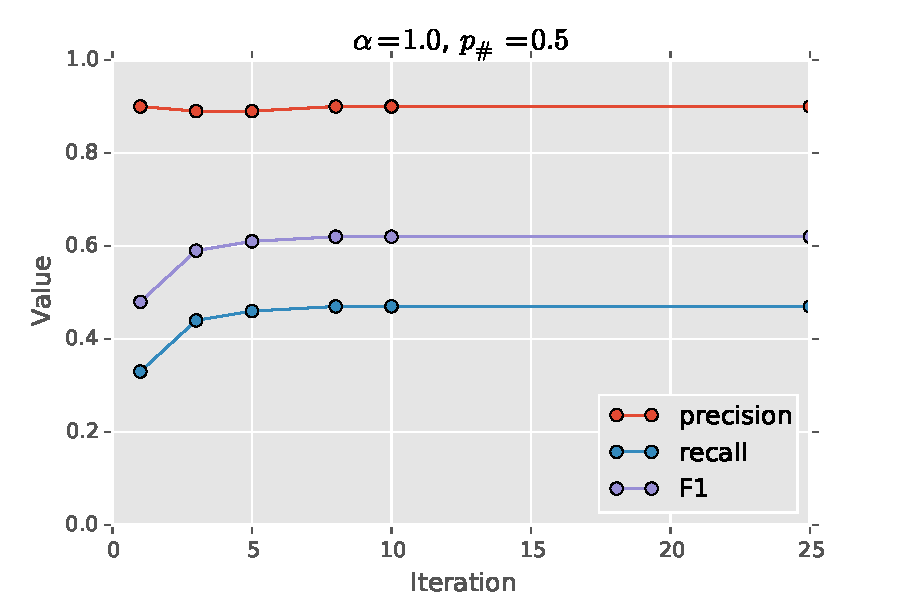
\includegraphics[width=0.5\textwidth]{fig/over_time_1_0_0_5.pdf}}}
  \subfloat[]{{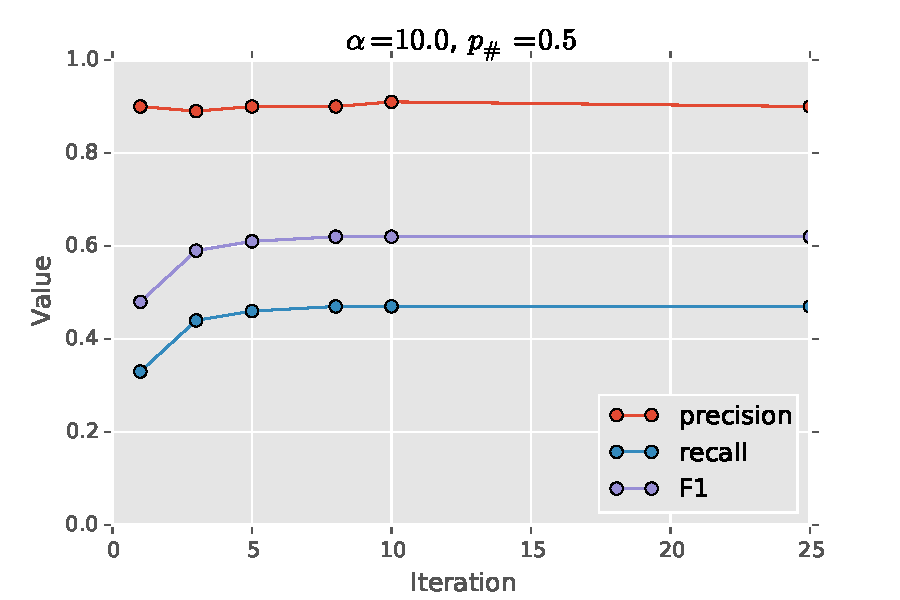
\includegraphics[width=0.5\textwidth]{fig/over_time_10_0_0_5.pdf}}}

  \subfloat[]{{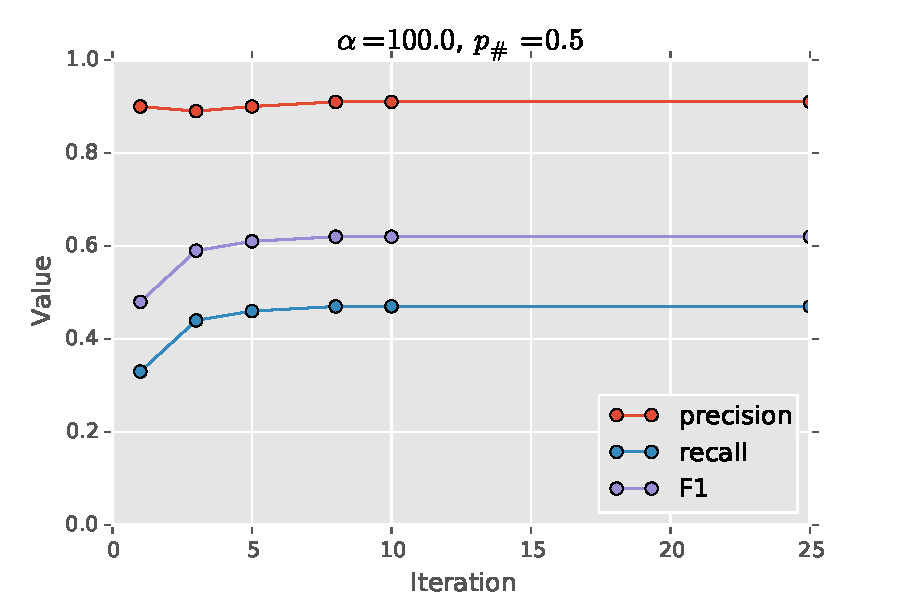
\includegraphics[width=0.5\textwidth]{fig/over_time_100_0_0_5.pdf}}}
  \subfloat[]{{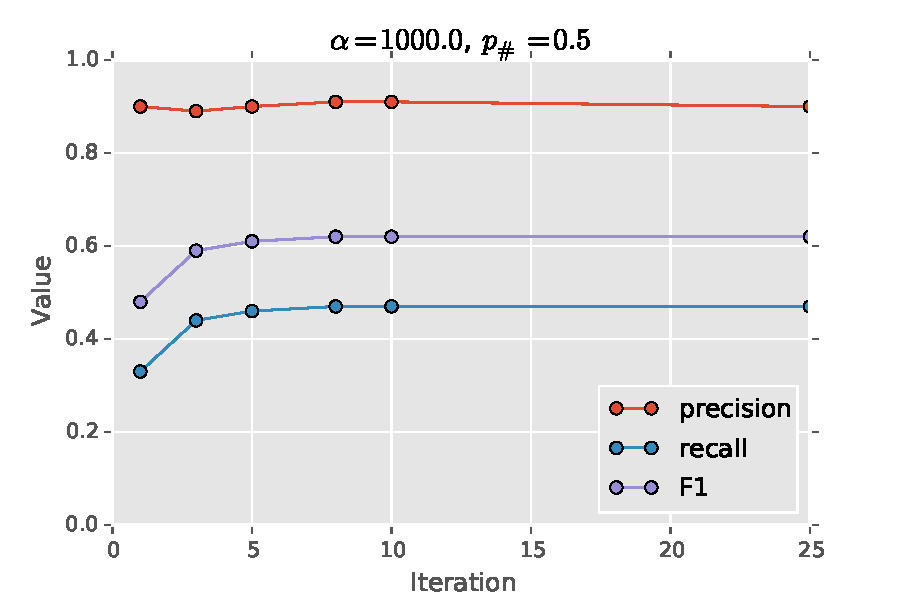
\includegraphics[width=0.5\textwidth]{fig/over_time_1000_0_0_5.pdf}}}

  \subfloat[]{{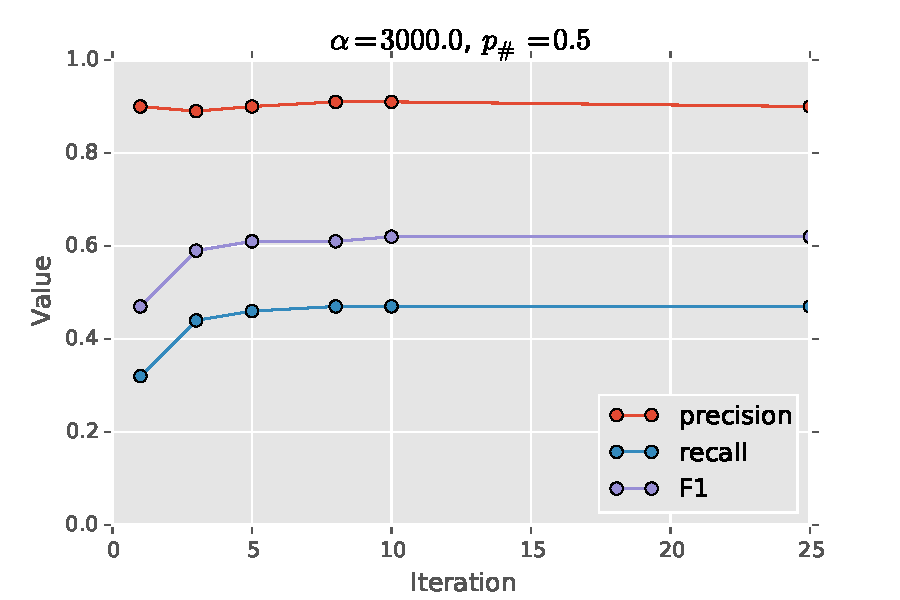
\includegraphics[width=0.5\textwidth]{fig/over_time_3000_0_0_5.pdf}}}
  \subfloat[]{{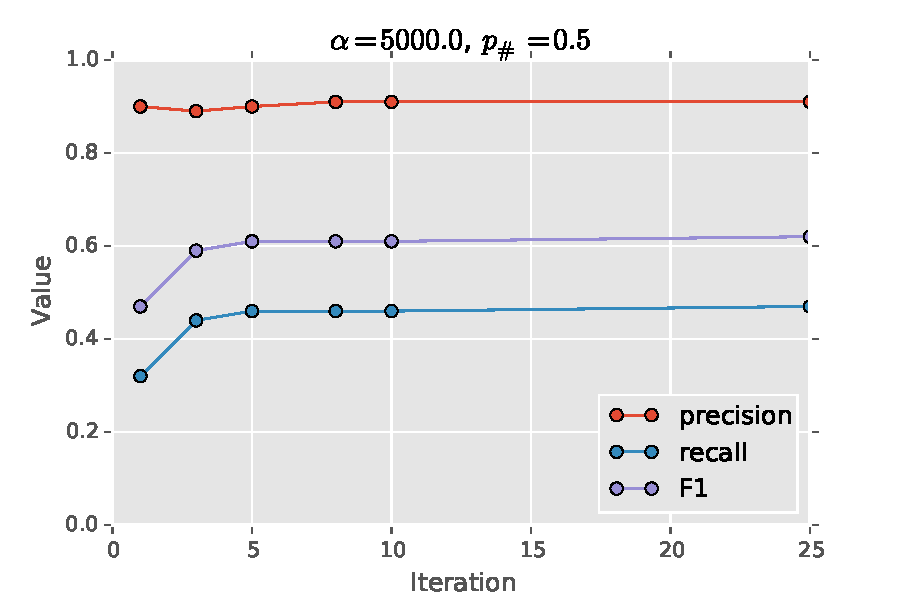
\includegraphics[width=0.5\textwidth]{fig/over_time_5000_0_0_5.pdf}}}

  \label{fig:iterations}
  \caption{Performance over iterations with $p_\# = 0.5$ and varying $\alpha$}
\end{figure}

\section{Conclusion}

\bibliographystyle{apalike}
\bibliography{report1}

\end{document}
